% Use pdfLatex to compile
\documentclass[aoas]{imsart}
\usepackage[dvipsnames]{xcolor}
\usepackage{charter}
\usepackage{latexsym,amssymb, amsmath, amsfonts}
\usepackage{graphicx} 
\RequirePackage{natbib}
%\usepackage{amsthm,wrapfig,url,bm,rotating,multirow}
\RequirePackage[colorlinks,citecolor=blue,urlcolor=blue]{hyperref}
%\RequirePackage{hypernat}

\startlocaldefs
\def\ci{\perp\!\!\!\perp}
%\def\bibfontsize{\small}
%\def\authorfmt#1{\textsc{#1}}
\def\MI{\textsf{MI}}
\def\PI{\textsf{PI}}
\def\KL{\textsf{KL}}
\def\ESS{\textsf{ESS }}
\def\Z{\textsf{Z}}
\def\BF{\textsf{BF}}
\def\M{{\cal{M}}}
\def\N{{\cal{N}}}
\def\P{{\cal{P}}}
\def\v{\mathbf{v}}
\def\ind{\thicksim}
\endlocaldefs

\graphicspath{{.}{Fig}}
\begin{document}

\begin{frontmatter}
\title{Adaptive Annealed Importance Sampling for Multi-Modal Posterior Exploration
  and Model Selection  with Application to Extrasolar Planet
  Detection\protect\thanksref{T1}}
\runtitle{AAIS for Exoplanet Detection}
\thankstext{T1}{This work has been supported by Statistical and
  Applied Mathematical Sciences Institute through National Science
  Foundation grant DMS--042240.  Any opinions, findings, conclusions
  or recommendations expressed in this material are those of the
  authors and do not necessarily reflect the views of the NSF.}

% Bin + Alphabetical authorship for now
\begin{aug}
\author{\fnms{Bin} \snm{Liu}\thanksref{t2,m1} \ead[label=e1]{bliu.81@gmail.com}},
\author{\fnms{Jim} \snm{Berger}\thanksref{t2,m1}\ead[label=e4]{berger@stat.duke.edu}},
\author{\fnms{Merlise A.}
  \snm{Clyde}\thanksref{t2,m1}\ead[label=e2]{clyde@stat.duke.edu}},
\author{\fnms{James L.}  \snm{Crooks}\thanksref{t2,m3}\ead[label=e5]{tba}},
\and
\author{\fnms{Tom} \snm{Loredo}\thanksref{t3,m2}\ead[label=e3]{loredo@cornell.edu}}


\thankstext{t2}{Partially supported by National Science Foundation Grant AST--0507481}
\thankstext{t3}{Partially supported by National Science Foundation
  Grant AST--XXXXX}
\runauthor{Liu et al.}

\affiliation{Duke University\thanksmark{m1}, Environmental Protection
  Agency\thanksmark{m3} and Cornell University\thanksmark{m2}}

\address{Department of Electrical and Computer Engineering \\
  Duke University \\
Durham, NC 27705 USA \\
  \printead{e1}}

\address{Department of Statistical Science \\
  Duke University \\
Durham, NC 27705 USA \\
 \printead{e2}\\
\phantom{E-mail:\ }\printead*{e4}}

\address{Department of Astronomy \\Cornell University \\
Ithaca, NY  USA \\
 \printead{e3}}
\end{aug}


\begin{abstract}
  The search for extrasolar planets presents several statistical
  challenges including model selection and inference within models
  that involve multi-modal posterior distributions.  To address these
  problems, we propose an adaptive annealed importance sampling
  algorithm (AAIS) which facilitates simulation from multi-modal joint
  posterior distribution and provides an effective and
  easy-to-implement method for estimating marginal likelihoods that
  are required for Bayesian model comparison.  Using a sequential
  importance sampling framework, we construct mixtures of Student $t$
  distributions to approximate a sequence of ``annealed''
  distributions that gradually approximates the target posterior
  density.  Borrowing ideas of birth/death and split/merge steps from
  reversible jump Markov-chain Monte Carlo, we propose an adaptive
  online method to increase/decrease the number of  mixture
  components guided by the effective sample size of the importance sample.
  We use simulation studies and several
  examples from exo-planet searches to demonstrate the greater
  efficiency of the method.
  The combination of annealing and heavier
  tails of the Student $t$ components in the mixture greatly
  facilitate capturing the ``spikey'' posterior densities present in
  the highly nonlinear models in the exo-planet problem, while importance sampling permits
  straightforward estimation of marginal likelihoods and posterior
  model probabilities to address the uncertainty of whether planets
  are indeed present.   We illustrate the methodology with several
  star systems and a simulation study.
\end{abstract}

\begin{keyword}
\kwd{Bayes Factor}
\kwd{Model Selection}
\kwd{Nonlinear Regression}
\end{keyword}

\end{frontmatter}


\section{Introduction}

Since the beginning of recorded time we have wondered whether we are
alone or whether there are other planets that might support life. The
scientific quest for extrasolar or exoplanets (planets beyond our own
solar system) began in the mid 19th century, but it was only as recent
as 1992 that astronomers have been able to confirm the existence of
other planetary systems.  Since then {\tt describe resources,
  telescopes, etc} have been devoted to identifying stars with
orbiting planets, and in particular, those that might have earth-like
planets. As of June 2010 over 450 exoplanets have been detected, the
majority using techniques that rely on measurements of a star's radial
velocity.  The presence of a planet orbiting a star will lead to a
periodic ``wobble'' in the the star's radial velocity, while if there
are no planets present the expected velocity is constant although
measurements fluctuate because of stellar jitter and other sources of
noise.  Based on a short sequence of noisy measurements, the challenge
is to determine whether there are no planets or one, two or more
planets, and if there are planets present to characterize their orbital
parameters.  {\tt cite work of Gregory and Ford, but mention
  limitations?}  If the data do not provide strong evidence either in
favor or against the presence of planets, additional observations may
be needed to provide confirmation.  Determining which stars to observe
and when to schedule scarce telescope time optimally is critical given
limited resources; Bayesian methods in particular are ideally suited
for updating information/evidence and decision
making in such sequential sampling problems.


The primary question of whether there are no planets or one or more
may be poised as a Bayesian model selection problem, where the
collection of models under consideration are the zero-planet mode
$\M_0$, one-planet $\M_1$, two-planet $\M_2$, etc.  In Bayesian
statistics, the posterior probability of a model $\M_j$ requires
accurately calculating the integrated or marginal likelihood ( see
\citet{Clyd:Geor:2004} for a general overview or
\citet{Clyd:etal:2005} for some of the issues that arise in
astronomy).  In the exoplanet application, each model $\M_p$ has
$2+5p$ parameters where $p$ is the number of planets, so even the
simplest single planet model requires a seven dimensional integral
over the parameter space to obtain the marginal likelihood.  Because
of the nonlinear nature of the models, analytic solutions do not
exist.  While low in dimension compared to many modern problems of
model selection, the models are highly nonlinear making Laplace
approximations untenable given the modest sample sizes and multi-modal
posterior distribution; constructing good proposal distributions for
Reversible Jump-Markov Chain Monte Carlo (RJ-MCMC) algorithms is near
impossible; just designing an efficient MCMC algorithm for sampling
from posterior distributions for a model with one planet is
challenging on its own due to the multi-modal nature of the posterior
distribution.  


Out of available methods for numerical integration,
importance sampling (IS) generally produces the best estimates of
marginal likelihoods in terms of bias and variance \citep{Christian's
  comparisons?}. The key to building an efficient IS algorithm is to
design an importance function that mimics the integrand.  Building
such a function can be quite challenging even in lower to modest
dimensional settings, with the multi-modal posterior distributions
that arise in the exoplanet setting the task is all the more
ambitious!  In this paper, we propose a novel adaptive method for constructing an
importance function using a mixture of Student-$t$ distributions that
evolves to the target posterior distribution.  The paper is organized
as follows.  We begin by presenting an overview of the radial velocity
models for exoplanet detection in Section
\ref{sec:exo} and discuss the scientific issues that inspired this
work. In Section \ref{sec:IS} we review importance sampling in the
context of calculating marginal likelihoods for Bayesian model
selection. In Section \ref{sec:AAIS} we present the Adaptive Annealed
Importance Sampling method developed for the exoplanet problem. This
method integrates several key features of other methods: mixture
models, annealing, and adaptation via a sequence of distributions to
build a flexible importance distribution that mimics the posterior
distribution, but incorporates ideas successfully used in
trans-dimensional methods to adapt the number of kernels in the
mixture by utilizing split and merge moves.  In Section
\ref{sec:simulation} we present two simulation studies that
demonstrate the efficiency of the method compared to other approaches.
The first involves a challenging flared helix in three dimensions,
while the second seven dimensional problem that was selected to reflex
the target function in the exoplanet problem.  In Section
\ref{sec:app} we illustrate the method in the analysis of several real
star systems with one and two planets. Finally, we conclude with
discussion of possible extensions of the method in Section
\ref{sec:disc}.



\section{Radial Velocity Models in the Search for Exoplanets}
\label{sec:exo}

In a two-body system such as a star and planet, the pair rotate
together about a point lying somewhere on the line connecting their
centers of mass. If one of the bodies (the star) radiates light, the
frequency of this light measured by a distant observer will
 vary  cyclically with a period equal to the orbital period. This
Doppler shift effect is understood well enough that astronomers can
translate between frequency shift and the star's velocity toward or
away from earth.  

If a star does not host any orbiting planets, then the radial velocity
(RV) measurements $v_i$ will be roughly constant over any period of time,
varying only due to the ``stellar jitter'' $s^2$, the random
fluctuations in a star's luminosity. Under the zero-planet
model, $\M_0$, the RV measurements are assumed to  have Gaussian distributions
\begin{equation}\label{0p_Model}
v_i \mid \M_0\ind \mathcal{N}\left(C,\sigma_i^2+s^2\right).
\end{equation}
with mean $C$, the constant center-of-mass velocity of the star
relative to the earth, and variances $\sigma^2_i + s^2$.  The
parameters $C$ and $s$ are both in the same units as the velocity
measurements, typically meters per second ($m/s$).  The additional
variance component $\sigma^2_i$ is a calculated error due to the
measurement procedure {\tt more
  details, ref, justification for additive form}.


The observed radial velocities (RV) $v_i$ at time $t_i$
for a single planet model, $\M_1$, are also assumed to be Gaussian
distributed  with
\begin{equation}\label{Velocity_Model}
v_i \mid \M_1 \ind \mathcal{N}\left(C_1 +\bigtriangleup
V(t_i|\phi_1),\sigma_i^2+s_1^2\right),
\end{equation}
where the velocity shift $\bigtriangleup
V(t_i|\phi_1)$ due to the presence of a single planet is
a  family of curves parametrized by the 5 dimensional vector
$\phi_1 \equiv (K_1,P_1,e_1,\omega_1,\mu_1)$
\begin{equation}\label{Velocity_1p_Model}
\bigtriangleup V(t|\phi_1)=K_1[\cos(\omega_1+T(t))+e\cos(\omega_1)]
\end{equation}
where $T(t)$ is the ``true anomaly at time $t$'' given by
\begin{equation}\label{true_anomaly}
T(t)=2\arctan\left[\tan(\frac{E(t)}{2})\sqrt{\frac{1+e_1}{1-e_1}}\right].
\end{equation}
and $E(t)$ is called the ``eccentric anomaly at time $t$'', which is the
solution to the transcendental equation
\begin{equation}\label{transcendental_equation}
E(t)-e_1\sin(E(t))=\mbox{mod}\left(\frac{2\pi}{P_1}t+\mu_1,2\pi\right).
\end{equation}
The five orbital parameters that comprise $\phi_1$ are the velocity
semi-amplitude $K_1$, the orbital period $P_1$, the eccentricity $e_1$,
$(0\leq e_1 \le 1)$, the argument of periastron $\omega_1$, $(0\le \omega
\le 2\pi)$ and the mean anomaly at time $t=0$, $\mu_1$, $(0\le \mu_1
\le 2\pi)$.  The parameters $C_1$ $K_1$ and $s_1$ have units $m/s$;
the velocity semi-amplitude $K_1$ is usually restricted to be
non-negative to avoid identification problems, while $C_1$ may be
positive or negative.  The eccentricity parameter $e_1$ is unit-less,
with $e_1 = 0$ corresponding to a circular orbit, and larger $e_1$ leading
to more eccentric orbits. Periastron is the point at which the planet
is closest to the star and the argument of periastron $\omega_1$, measures
the angle at which we observe the elliptical orbit.  The mean anomaly $\mu_1$ is
an angular distance of a planet from periastron. 

If there are $\P \ge 1$ planets, the expected velocity is given by $C_p
+ \bigtriangleup V(t_i|\phi_1,\ldots,\phi_p)$ with the overall velocity shift
$\bigtriangleup V$  approximated as the sum of the velocity
shifts of the individual planets:
\begin{equation}\label{Velocity_2p_Model}
\bigtriangleup V(t_i|\phi_1,\ldots,\phi_p)=\sum_{j=1}^p
K_j[\cos(\omega_j+T_i(t_i))+e_j\cos(\omega_j)]
\end{equation}
where the planets' mutual gravitational interactions are assumed to be
negligible.  With $p$ planets, there are a total of $2+5p$ parameters,
$\theta_p = \{ \mathcal{C_p},s_p^2,\phi_1,\ldots,\phi_p\}$ for each of
the models $\M_p$, $p \in \{0, 1, \ldots \P\}$. Of course, we do not
know how many planets there are \emph{a priori} - indeed, finding the
number of planets $p$ and characterizing their orbital parameters is
a major aim.

\subsection{Bayesian Methods for Identifying the Number of Planets}
Determining the number of planets in a
system is, from a statistical point of view, a model choice
problem. Bayesian model selection requires calculation of marginal
likelihoods of models or ``evidence'' provided by the data for each model:
\begin{equation}\label{marginal_lik}
m( \M_p) = \int_{\Theta_p}
p(\v \mid \theta_p,\M_p) p(\theta_p \mid \M_p) d\theta_p
\end{equation} 
which entails integrating the sampling model of the
data $\v = (v_1, \ldots v_n)^T$ with respect to the prior distribution
of model specific parameters $\theta_p$.
Bayes Factors for comparing a $p$ planet model to the $0$ planet model
may be expressed  as
\begin{equation}
\BF(\M_p:\M_0)=\frac{m( \v \mid \M_p)}{m(\v \mid \M_0)}
\end{equation}
where the Bayes factor $\BF(\M_0,\M_0) = 1$,
while the posterior probability of the $p$ planet model is of the
form
\begin{equation}
  \label{eq:post-prob}
  p(\M_p \mid \v) = \frac{\BF(\M_p:\M_o) O(\M_p: \M_0)} 
{ \sum_{ j= 1}^{p_{\max}} \BF(\M_j:\M_o) O(\M_j: \M_0)}
\end{equation}
where $O(\M_p: \M_0)$ is the prior odds of having $p$ planets to $0$
planets and $p_{\max}$ is the maximum number of planets for the
system.  This requires specifying a prior distribution on $\theta_p$
for each of the models in order to obtain marginal likelihoods and
Bayes factors.

\subsection{Priors Distributions}
We adopt the prior distributions recommended by \cite{ford2006bms, bullard2009edc},
which are based in part on their approximate realism, but also their
mathematical tractability.  For all models, intercept parameter
$C_p$ and stellar jitter parameter $s_p$, are taken as
being {\it a priori} independent, where $C_p$ is uniform over a finite
set $[C_{\min}, C_{\max} ] $
\begin{subequations}
\begin{align}
\label{prior_C}
p_C(C) & =\left\{\begin{aligned}
\frac{1}{C_{\max}-C_{\min}} &~ \qquad\qquad\qquad\mbox{for } ~C_{\min}\leq C\leq C_{\max}\\
0\quad\quad &~ \qquad\qquad\qquad\mbox{otherwise}  \\
\end{aligned}
\right. 
\intertext{and  $\log(s_{\min} + s_p)$ has a   uniform distribution on
the interval $(\log(s_{\min}), \log(s_{\max})]$, }
\label{prior_sigma}
p_{s}(s) &  = \left\{\begin{aligned}
\frac{1}{ \log \left(1+\frac{s_{\max}}{s_{\min}}\right)} \cdot \frac{1}{s_{\min}+s}
&~ 
\quad\quad\mbox{for } ~0 < s \leq s_{\max} \\
0 \quad\quad &~ \quad\quad\mbox{otherwise.}  \\
\end{aligned} \right.
\end{align}
\end{subequations}
The joint prior on $(C_p, s_p)$ may be viewed as  a
modified independent Jeffrey's prior  as $C_{\min} \to -\infty$,
$C_{\max} \to \infty$, $s_{\min} \to 0$, $s_{\max} \to \infty$, which leads
to well defined posterior distributions and Bayes Factors even in the limit. 

For each of the $p$ planet models, in the absence of other prior
information, we take each $\phi_j$ to have independent identical prior
distributions.  Many of the parameters in $\phi_p$ allow informative
marginal prior distributions to be specified, however, the nonlinear
relationships induce strong correlations among many of the parameters,
which leads to a difficult task for joint prior elicitation.  For
circular orbits ($e = 0$), $\omega$ and $\mu_0$ are in fact
unidentifiable.  To simplify this task, we specify independent prior
distribution for the components of each $\phi_p$ in a transformed
parameter space,
$$
\begin{aligned}
  x & = e\cos\omega  \label{eq:poincare-x} & \quad &   y & =
  e\sin\omega \label{eq:poincare-y} & \quad & z & = (\omega+\mu_0)
  \mod 2\pi \\
  \dot{P} & = \log P  & \quad &  \dot{K} & = \log K &  \quad & 
\end{aligned}
$$
leading to  $\dot{\phi}_p \equiv (\dot{K}_p, \dot{P}_p, x_p, y_p, z_p)^T$.  The 
Poincar\'e variables $x_p$ and $y_p$   greatly reduce the very
strong correlations between $\mu_p$ and $\omega_p$, which  is particularly
important for low eccentricity orbits, where the parameters are nearly
unidentifiable.  The use
of  $z$ further reduces correlations between the 
parameters $\omega$ and $\mu_0$ when $e\ll1$, but has little effect
for large $e$.  \citet{bullard2009edc} recommended using the log
transformation of $P$ and $K$ 
as  posterior distributions were  more Gaussian in these
coordinates, which led to improved posterior simulation. 
In the transformed parameter space, the prior distribution for $\phi$
is 
\begin{subequations}
\begin{equation}\label{prior_1p}
p_{\dot{\phi}}(\dot{\phi})=c_\phi \cdot\exp\dot{K}\cdot\frac{1}{1+\frac{\exp\dot{K}}{K_{\min}}}\cdot\frac{1}{\sqrt{x^2+y^2}}
\end{equation}
for $\log(K_{\min}) < \dot{K} \leq\log(K_{\max})$,
$\log(P_{\min})\leq\dot{P}\leq\log(P_{\max})$, $x^2+y^2<1$, and $0\leq
z\leq2\pi$,
where the normalizing constant is 
\begin{equation}\label{kappa_in_prior_1p}
c_\phi
=\frac{1}{\log\left(1+\frac{K_{max}}{K_{\min}}\right)}\cdot\frac{1}{K_{\min}}\cdot\frac{1}{\log\left(\frac{P_{\max}}{P_{\min}}\right)}\cdot\left(\frac{1}{2\pi}\right)^2. 
\end{equation}
\end{subequations}
The constants in the prior distribution (see Table \ref{tab:hyper}) are set based upon the physical realities
(e.g., an orbit with too small a period will result in the planet
getting consumed by the star) \citep{bullard2009edc}
\begin{table}[h]
  \begin{center}
  \begin{tabular}{|lr|lr|} \hline \hline
$P_{\min}$ &  $1$ day &
$P_{\max}$ &  $1,000$ years \\
$K_{\min}$ &  $ 1$ m/s & 
$K_{\max}$ &  $2128$ m/s \\
$C_{min}$ &  $-2128$ m/s & 
$C_{max}$ &   $2128$ m/s \\
$s_{\min}$ &  $1$ m/s &
$s_{\max}$ &  $2128$ m/s \\ \hline
  \end{tabular}
  \end{center}
\caption{Prior hyperparameters for the distribution of $\phi_p$.}
\label{tab:hyper}
\end{table}
 of the form given in \ref{prior_1p}
with hyperparameters from Table \ref{tab:hyper}.


\section{Importance Sampling for Marginal Likelihood Estimation}
\label{sec:IS}
Beyond conjugate models, the integrals defining the marginal
likelihood in Equation (\ref{marginal_lik}) are generally intractable
and must be estimated by numerical methods.  Importance sampling (IS)
\citep{Gewe:1989} is a well known Monte Carlo technique for estimating
integrals, where
the marginal likelihood may be re-expressed as an expectation with
respect to  an importance distribution $Q$ that is
abolutely continuous with respect to the target posterior distribution
\begin{equation}\label{IS_for_marginal_lik}
m(\M ) = \mathbb{E}_Q\left[ \frac{p(\v \mid \theta, \M)p(\theta \mid 
    \M)} {q(\theta)}\right]
\end{equation}
and the ``importance function'' $q(\theta)$ is the associated probability
density function for 
distribution $Q$.  Ideally it should be straight-forward to generate 
a sample of size $N$,  $\theta^{(1)},
\ldots, \theta^{(N)}$ from $Q$, leading to 
an  unbiased and simulation consistent Monte Carlo
estimate of the marginal likelihood
\begin{equation}\label{IS_solution_marlik}
\hat{m}(\M)=\frac{1}{N} \sum_{i=1}^N\frac{p(\v \mid \theta^{(i)},
  \M) p(\theta^{(i)}\mid \M)} {q(\theta^{(i)})} = \frac{1}{N}\sum_{i=1}^N
w^{(i)} = \bar{w}
\end{equation}
where $w^{(i)}$ are known as the IS weights. 
The variance of the IS estimator is
\begin{subequations}
\begin{align}
\mbox{Var}_Q\left[\hat{m}(\M) \right] & =\frac{\sigma_q^2}{N} 
\intertext{where}
\sigma_q^2 &
=\mbox{Var}_q\left\{\frac{p(\v \mid \theta, \M)p(\theta|\M)}{q(\theta)}\right\}\\
%& =\int_{R^d}\left(\frac{p(\v \mid \theta, \M)p(\theta|\M)}{q(\theta)}-m(\M)\right)^2
%q(\theta)d\theta\\
& =m(\M)^2\int \left(\frac{\pi(\theta
 \mid \v, \M)-q(\theta)}{q(\theta)}\right)^2 \, q(\theta)\, d\theta
\intertext{
where  a consistent estimator of $\sigma_q^2$ is the
usual variance}
\hat{\sigma}_q^2 & \simeq\frac{1}{N}\sum\limits_{i=1}^N\left(w^{(i)}-\bar{w}\right)^2.
\end{align}
\end{subequations}

The efficiency of importance sampling depends largely on how close the
importance function mimics the shape of the target distribution,
$\pi(\theta \mid \v, \M)$ which is proportional to $p(\v \mid \theta,
\M) p(\theta \mid \M)$.  If the importance function has lighter tails
than the target, the estimate will tend to be unstable because the
weights can be arbitrarily large; on the other hand if the importance
function has much fatter tails than the target, too many of the
$\theta_i$'s will be drawn from the tails, resulting in a seemingly
stable estimate, but with many small weights.  These problems are only
compounded in high-dimensional settings.


\section{Annealed Adaptive IS Method for Constructing Importance
  Function} \label{sec:AAIS}
In this section, we propose the adaptive mixture modeling approach,
which is used for constructing importance function that resembles
the posterior and then is used in (\ref{IS_solution_marlik}) for
calculating the marginal likelihood.

Let $\pi(\theta)$ denote the posterior distribution, which is
proportional to $L(y|\theta)p(\theta)$. Note that computing
$L(y|\theta)p(\theta)$ for any $\theta$ is feasible, but that we are
not able to directly sample from the distribution it defines, i.e.
$\pi(\theta)$. The aim is to find a distribution, $q(\theta)$, that
approximates $\pi(\theta)$, which we are also able to evaluate.

We first select an initial proposal distribution $q_0(\theta)$, then
define a series of intermediate distributions between $q_0(\theta)$
and $\pi(\theta)$, by
\begin{equation}
\pi_t(\theta)\propto
q_0(\theta)^{1-\lambda_t}\pi(\theta)^{\lambda_t}, \quad\quad
t=1,\ldots,T, \quad \mbox{and}\quad
0<\lambda_1<\lambda_2<\dots<\lambda_T=1.
\end{equation}
Finally we propose an iterative method to construct $q(\theta)$, as
shown in Algorithm 1.
\begin{center}
\textbf{Algorithm 1. Sequential Proposal Construction}
\end{center}
\begin{itemize}
\item Use $\pi_1(\theta)$ as the target distribution, with $q_0(\theta)$
as the proposal. Tune parameters of $q_0(\theta)$ to obtain an
updated mixture density function, denoted $q_1(\theta)$, which
approximates $\pi_1(\theta)$.
\item Similarly as in step 1, tune parameters of $q_1(\theta)$ to
obtain an updated proposal,$q_2(\theta)$, which is used to
approximate $\pi_2(\theta)$.
\item iterates the above process, i.e., tuning parameters of $q_t(\theta)$ and then getting the updated mixture density function $q_{t+1}(\theta)$, from $t=2$ to $t=T-2$.
\item Use $\pi_T(\theta)$ as the target distribution, tune parameters of
$q_{T-1}(\theta)$ to obtain $q_{T}(\theta)$, which approximates
$\pi_T(\theta)=\pi(\theta)$. Then $q_{T}(\theta)$ is actually the
importance function which we want.
\end{itemize}

We see that the annealing strategy is adopted in the above iterative
procedure. In what follows, we propose an adaptive method to handle
the task of updating $q_{t-1}(\theta)$ to $q_{t}(\theta)$ in
Algorithm 1.

\subsection{Multivariate Student's T-mixture Model}
Considering possible complexities in the structure of
$\pi_t(\theta)$, we employ a mixture model to define
$q_{t}(\theta)$. Note that any continuous probability density
function can be approximated by a finite mixture model, provided
that the mixture has a sufficient number of components along with
correctly estimated parameters
\citep{bishop2005neural,zeevi1997det}. In particular, we equip
$q_{t}(\theta)$ with the Student's T distribution as the mixture
component, making it easier to detect modes that are far apart
thanks to its fat tail structure. Let $\mathcal{S}_d(\mu,\Sigma,v)$
denote a $d$-variate Student's T distribution, where $\mu$ is the
center, $\Sigma$ the positive definite inner product matrix, and $v$
is the degrees of freedom. We just fix $v$ to be a constant, e.g., 5
in the following. So the mixture model we use is:
\begin{equation}\label{Definition_mixture}
q(\theta|\psi)=\sum\limits_{m=1}^M \alpha_{m}
\mathcal{S}_d(\theta|\mu_m,\Sigma_m)
\end{equation}
where
$\psi=\{M,\alpha_1,\ldots,\alpha_M,\mu_1,\ldots,\mu_M,\Sigma_1,\ldots,\Sigma_M\}$
is the mixture parameter. Here $\alpha_m$ is the probability mass of
the $m$th component. It satisfies that $\alpha_{m}\geq
0,\sum_{m=1}^M \alpha_{m}=1$. So the task of fitting a T-mixture
model to a probability density translates into seeking suitable
parameter values for $\psi$.

\subsection {Proposal Adaptation via IS plus EM}\label{sec:IS_EM}
Let's focus on iteration $t$ in Algorithm 1. We first simulate an
random sample, $\theta^n$, from $q_{t-1}(\theta)$, with the
importance weight calculated by
\begin{equation}
w^n=\frac{\frac{\pi_{t}(\theta^n)}{q_{t-1}(\theta^n)}}{\sum_{n=1}^N\frac{\pi_{t}(\theta^n)}{q_{t-1}(\theta^n)}},
\end{equation}
where $N$ denotes the sample size. The resulting weighted particle
set then can be seen as a particle approximation to the current
target distribution $\pi_t(\theta)$, i.e.
\begin{equation}\label{delta_mass_approx}
\pi_t(\theta)\simeq\sum\limits_{n=1}^Nw^i\delta(\theta^i),
\end{equation}
where $\delta(\cdot)$ is the delta mass function.

Here we adopt the Kullback-Leibler (KL) divergence to measure the
distance between any two distributions. Then the aim is to obtain a
proposal, $q_t(\theta)$, that minimizes the KL distance with respect
to $\pi_t(\theta)$, which is shown to be
\begin{equation}\label{KL}
\mathcal{D}[\pi_t(\theta)||q_t(\theta|\psi)]=\mathbb{E}_{\pi_t(\theta)}\left[\log\frac{\pi_t(\theta)}{\sum\limits_{m=1}^M
\alpha_m\mathcal{S}_d(\theta|\mu_m,\Sigma_m)}\right].
\end{equation}
where $\mathbb{E}_f$ denotes expectation with respect to a function
$f$. It's clear that minimizing (\ref{KL}) in $(\alpha,\mu,\Sigma)$
is equivalent to maximizing
\begin{equation}\label{MLE}
\int\pi_t(\theta)\log\left(\sum\limits_{m=1}^M
\alpha_m\mathcal{S}_d(\theta|\mu_m,\Sigma_m)\right).
\end{equation}
Substituting Equation (\ref{delta_mass_approx}) in the above, we
have
\begin{equation}\label{Max_log_lik}
\sum_{i=1}^N w^i\log\left(\sum\limits_{m=1}^M
\alpha_m\mathcal{S}_d(\theta^i|\mu_m,\Sigma_m)\right).
\end{equation}

At this stage, the task translates into a mixture-density parameter
estimation problem, that is, how to optimize the parameter values of
$\psi$ to make the resulting mixture density function fit the data
$\{\theta^n,w^n\}_{n=1}^N$ as well as possible.

Given data component $\theta^n$, the posterior probability of each
mixture component can be obtained according to the Bayes rule:
\begin{equation}\label{posterior_prob_component}
\rho_m(\theta^n)=\alpha_m
\mathcal{S}_d(\theta^n;\mu_m,\Sigma_m)/q(\theta^n),
\end{equation}
where $\alpha_m$ is regarded as the prior, and
$\mathcal{S}_d(\theta^n;\mu_m,\Sigma_m)$ is the associated
likelihood. The proportion mass of this component can then be
updated by
\begin{equation}\label{MLE_alpha}
\alpha_m=\sum\limits_{n=1}^N w^n \rho_m(\theta^n).
\end{equation}
And each pair of $\{\mu_m,\Sigma_m\}$ can be updated by the
following Equations:
\begin{equation}
\mu_m=\frac{\sum\limits_{n=1}^N w^n
\rho_m(\theta^n)u_m(\theta^n)\theta^n}{\sum\limits_{n=1}^N w^n
\rho_m(\theta^n)u_m(\theta^n)},
\end{equation}
\begin{equation}\label{MLE_Sigma}
\Sigma_m=\frac{\sum\limits_{n=1}^N w^n
\rho_m(\theta^n)u_m(\theta^n)C_n }{\sum\limits_{n=1}^N w^n
\rho_m(\theta^n)},
\end{equation}
where
\begin{equation}
u_m(\theta)=\frac{v+d}{v+(\theta-\mu_m)^T(\Sigma_m)^{-1}(\theta-\mu_m)}
\end{equation}
and $C_n=(\theta^n-\mu_m)(\theta^n-\mu_m)'$, where $'$ denotes
matrix transposition.

The operations from (\ref{posterior_prob_component}) to
(\ref{MLE_Sigma}) constitute one iteration of the EM algorithm,
which is used to do mixture density parameter estimation
\citep{peel2000rmm}. Let $q_t(\theta)$ be a T-mixture model, with
the updated parameter values $\{\alpha_m,\mu_m,\Sigma_m\}$, and it's
expected to be an approximation to $\pi_t(\theta)$. The efficiency
of $q_t(\theta)$, as an approximation of $\pi_t(\theta)$, can be
measured by the KL divergence using (\ref{Max_log_lik}), or the
effective sample size, which is defined to be
\begin{equation}\label{ESS}
\ESS=\frac{1}{\sum_{n=1}^N w_n^2}.
\end{equation}
Note that these importance weights are associated with the random
sample drawn from $q_t(\theta)$. The \ESS was originally proposed by
\cite{kong1994sequential} to measure the overall efficiency of an IS
algorithm. Heuristically it measures how many i.i.d samples are
equivalent to the $N$ weighted samples. The \ESS is related to the
coefficient of variation (CV) of the importance weights (see
\cite{kong1994sequential}), which finds applications in
\cite{ardia2008adaptive,cappe2008ais,cornebise2008adaptive}. It's
shown that \ESS is determined by the associated proposal and the
particle size, $N$, while, once $N$ is big enough, the ratio of \ESS
to $N$ should be stable. So in this paper, we use \ESS$/N$ as a
quantity to monitor the efficiency of $q_t(\theta)$. When \ESS$/N$
is big enough, let Algorithm 1 go to next iteration. If \ESS$/N$ is
smaller than a given threshold, we continue to update $q_t(\theta)$
until it satisfies the requirement, i.e. the resulting \ESS$/N$ is
big enough. In this way, we can make sure that the finally obtained
$q_t(\theta)$ is really a good approximation to $\pi_t(\theta)$.

Suppose that currently \ESS$/N$ is not big enough, we consider two
approaches that are used to update $q_t(\theta)$ again. First we
check whether the particle with the biggest importance weight,
denoted $\theta^{W}, W\in\{1,\ldots,N\}$, is located in the tail of
the proposal. If it is, which means $q_t(\theta^{W})$ is smaller
than the proposal densities of most other particles, we then select
to perform an operation called component-splitting (see Section
\ref{sec:split}), otherwise, we perform the IS plus EM procedure
again. The reason for doing this is that the IS plus EM procedure is
exactly a local search approach, because it fixes the number of
mixture components to be a constant and the EM itself is a local
optimization method, while the component-splitting procedure will
break the local model structure by splitting one mixture component
into two, thus facilitates to find the global or, at least a better
local optimum (see Section \ref{sec:split}).


\subsection {Online Approach to Tune the Number of the Mixture Components}

In the above IS plus EM procedure, the number of components $M$ is
imposed to be constant, while this assumption is of course not
reasonable. To deal with this issue, we propose a series of adaptive
mechanisms to adapt $M$ online, which include operations called
components-merging, components-splitting and components-deletion,
respectively. We'll provide respective conditions, on which each of
these procedures needs to be performed.

\subsubsection{Components Merging}
This step targets for merging mixture components that have much
mutual information among each other. To begin with, we first
introduce the concept, mutual information. Suppose that a set of
equally weighted data components $\{\theta^n\}_{n=1}^N$ are
available, whose distribution is modeled by a mixture density
function $q=\sum_{m=1}^M\alpha_mf_m$. Given any data component
$\theta^n$, the posterior probability of each mixture component
$f_m$ can be calculated by
\begin{equation}
\rho_m(\theta^n)=\alpha_m f_m(\theta^n)/q(\theta^n).
\end{equation}
If there are two mixture components $f_i$, $f_j$, for which it
satisfies that $\rho_i(\theta^n)=\rho_j(\theta^n)$ for any
$n\in\{1,\ldots,N\}$, then $f_i$ and $f_j$ are regarded to contain
completely overlapped information. Inspired by the components
merging criterion proposed in \cite{ueda2000sam,wang2004estimation},
we define the mutual information between $f_i$ and $f_j$ to be:
\begin{equation}\label{mutual_info}
\MI(i,j)=\frac{(\Upsilon_i-\bar{\Upsilon}_i)^T(\Upsilon_j-\bar{\Upsilon}_j)}{\|\Upsilon_i-\bar{\Upsilon}_i\|\cdot\|\Upsilon_j-\bar{\Upsilon}_j\|},
\end{equation}
 where
$\Upsilon_m=[\rho_m(\theta^1),\ldots,\rho_m(\theta^N)]'$, $'$
denotes transposition of a matrix, $\|\cdot\|$ denotes the Euclidean
norm, and $\bar{\Upsilon}_m=\frac{1}{N}\sum_{n=1}^N
\rho_m(\theta^n)\textbf{1}_N$. Here $\textbf{1}_n$ denotes the
$n-$dimensional column vector with all elements being $1$.

Note that $\MI(i,j)\in[-1,1]$, and $\MI(i,j)=1$ iff $f_i$ and $f_j$
contain completely overlapped information.

In our algorithm framework, each data point $\theta^n$ is weighted
by $w^n$. Accordingly, $\Upsilon_m$ should be $\sum_{n=1}^N w^n
\rho_m(\theta^n)$, and the mutual information between $i$, $j$ turns
out to be:
\begin{equation}\label{Merge_criterion_correlation}
\MI(i,j)=\frac{(\Upsilon_i-\bar{\Upsilon}_i)'
D(w)(\Upsilon_j-\bar{\Upsilon}_j)}{\sqrt{\sum_{n=1}^N
w^n(\Upsilon_i(\theta^{n})-\bar{\Upsilon}_i)^2}\sqrt{\sum_{n=1}^N
w^n(\Upsilon_j(\theta^{n})-\bar{\Upsilon}_j)^2}}
\end{equation}
where
\begin{equation}
D(w)=diag([w^1,\ldots,w^N])
\end{equation}
We judge if two components, $i$ and $j$, need to be merged into one
by comparing $\MI(i,j)$ with a threshold $0<T_{merge}<1$. If
$\MI(j,k)>T_{merge}$, we then merge the $i$th component into $j$,
and set $M=M-1$; otherwise, we maintain the original mixture. The
merging operation is specified to be:
\begin{eqnarray}\label{Linear_combination_components}
\alpha_{j}&=&\alpha_{i}+\alpha_{j}\\
\mu_{j}&=&\frac{\alpha_{i}\mu_{i}+\alpha_{j}\mu_{j}}{\alpha_{j}}\\
\Sigma_{j}&=&\frac{\Sigma_{i}\mu_{i}+\Sigma_{j}\mu_{j}}{\alpha_{j}}
\end{eqnarray}
which is a linear combination of the two old components, and has
been used in \cite{wang2004estimation}. We traverse each pair of the
original components to do the merging judgements and perform the
above merging operation if the merging condition satisfies.

We execute the above merging operation when superfluous components
may exist, e.g., when $q_0(\theta)$ is initialized with too many
overlapped components, or too many new components appear at one
iteration of Algorithm 1 via component-splitting (see Section
\ref{sec:split}).

\subsubsection{Component-splitting}\label{sec:split}
As mentioned in Section \ref{sec:IS_EM}, it may happen that, after
performing the IS plus EM procedure, \ESS$/N$ was not big enough,
and the maximum weight particle was located in the tail of
$q_t(\theta)$. In that case, we perform the mechanism proposed here,
called component-splitting. This procedure is used to break the
local structure of $q_t(\theta)$ by splitting one component into
two, whereby the component number, $M$, will increase to $M+1$.

This Component-splitting approach is performed as follows. First,
when we simulate draws from $q_t(\theta)$ for evaluating the
efficiency of $q_t(\theta)$, we record the component origination of
each draw. We then see the parent component of the maximum weight
sample, $\theta^W$, denoted
$f_p=\mathcal{S}_d(\theta|\mu_p,\Sigma_p)$, and know that which
samples were originated from $f_p$. We encapsulate the samples that
come from $f_p$ to a data array,
$\mathcal{\theta}_{local}=\{\theta^{1},\ldots,\theta^{pN}\}$, then
split $f_p$ into two components$-$
$f_{c1}=\mathcal{S}_d(\theta|\mu_{c1},\Sigma_{c1})$ and
$f_{c2}=\mathcal{S}_d(\theta|\mu_{c2},\Sigma_{c2})$, and finally
replace $f_p$ in $q_t(\theta)$ by $f_{c1}$ and $f_{c2}$.

Next we give operations to get
$\mu_{c1},\Sigma_{c1},\mu_{c2},\Sigma_{c2}$. We first initialize
$\mu_{c1}=\theta^W$, $\mu_{c2}=\mu_p$,
$\Sigma_{c1}=\Sigma_{c2}=\Sigma_p$, and then specify a local mixture
$q_{local}=\alpha_{c1}f_{c1}+\alpha_{c2}f_{c2}$, where
$\alpha_{c1}=\alpha_{c1}=0.5$, finally we perform a local IS plus EM
procedure to update
$\alpha_{c1},\alpha_{c2},\mu_{c1},\Sigma_{c1},\mu_{c2},\Sigma_{c2}$.
Such local IS plus EM procedure starts by evaluating the local
weight for each $\theta^{i}$ in $\mathcal{\theta}_{local}$ via
\begin{equation}
w^i=\frac{\frac{\pi_{t}(\theta^{i})}{q_{local}(\theta^{i})}}{\sum_{n=1}^{pN}\frac{\pi_{t}(\theta^n)}{q_{local}(\theta^n)}}.
\end{equation}
Substituting $\{\theta^i,w^i\}_{i=1}^{pN}$ and the local mixture
parameters,
$\alpha_{c1},\alpha_{c2},\mu_{c1},\Sigma_{c1},\mu_{c2},\Sigma_{c2}$
in the Equations from (\ref{MLE_alpha}) to (\ref{MLE_Sigma}), we
then can obtain the updated parameter values for the local mixture
$q_{local}$. Suppose that $f_p$ is assigned a proportion mass
$\alpha_p$ in $q_t(\theta)$, we assign $f_{c1}$ and $f_{c2}$
proportion masses $\alpha_{c1}=\alpha_p\alpha_{c1}$ and
$\alpha_p\alpha_{c2}$, respectively, for the updated $q_t(\theta)$,
in which $f_p$ is replaced by $f_{c1}$ and $f_{c2}$.

This component-splitting method makes use of the local behavior of
the target distribution around the maximum weight sample. It adds
mixture proposal probability mass to those areas of the parameter
space which is near the maximum weight sample, where there is
relatively little mixture proposal probability mass. As the local IS
plus EM procedure is actually a local mixture learning process, by
which the local structure around the maximum weight sample will be
modeled well by the updated local mixture, which then will elicit a
better global mixture representation of the whole target
distribution, which may lead to a satisfactory \ESS$/N$ value. Note
that the above component-splitting procedure may be repeated
provided that the condition of executing it satisfies.

\subsubsection{Component-Deletion} \label{sec:deletion}
As mentioned above, when simulating draws from $q_t(\theta)$, we can
record the component origination of each sample. For any mixture
component that generates no sample, we deem it has taken no effect
in modeling the current target distribution, thus we just delete it
in current mixture proposal. Its probability masses is then
redistributed strengthening the remaining components.

\subsection{Practical Issues to be Considered}
EM based mixture modeling approach provides a convenient and
flexible utility for estimating or approximating distributions,
while the mixture log-likelihood presents a well known problem,
i.e., degeneracy toward infinity \citep{biernacki2003degeneracy}
(actually EM also suffers from the problem of slow convergence, so
it may converge to a local optimum \citep{biernacki2003degeneracy},
however, we don't need to worry about that, because on one side the
proposed component-splitting procedure facilitates to search the
global optimum, and, one the other side, the objective here is just
to find a good mixture importance function, which is not necessary
to be the global optimum). To prevent the mixture log-likelihood
from arising to infinity, we assign an inverse-wishart prior on the
covariance matrix of each mixture component, then perform EM to get
the \emph{maximum a posterior} (instead of maximum likelihood)
estimate of the covariance matrix.

In the component-splitting step, the parameter updating of $f_{c1}$
and $f_{c2}$ is based upon $pN$ particles originated from $f_p$. In
case of $pN$ being too small, e.g. smaller than a threshold
specified beforehand, denoted $N_s$, we need to generate another set
of $N_s-pN$ samples from $f_p$, then do the parameter updating for
$f_{local}$ based upon the $N_s$ particles. By doing this, we can
guarantee that we are using a sufficient number of random draws to
capture the local structure in the posterior, that will then be
represented by $f_{local}$.

In the above mentioned component-splitting step, when we replace
$f_p$ in $q_t(\theta)$ by $f_{c1}$ and $f_{c2}$, we assign the
proportion mass of $f_p$ to $f_{c1}$ and $f_{c2}$ proportionally to
their original weights, i.e. $\alpha_{c1}$ and $\alpha_{c2}$,
respectively. Note that if $\alpha_p$ is a very small value, e.g.,
$0.0001$, the new added mixture components, $f_{c1}$ and $f_{c2}$,
will only take an insignificant effect in the updated $q_t(\theta)$,
while $f_{c1}$ and $f_{c2}$ may contain new and important
information about the posterior. To guarantee that $f_{c1}$ and
$f_{c2}$ can play a role in $q_t(\theta)$, at lease to some extent,
we propose the following operations. We first specify a threshold
$\alpha_{threshold}$, which may be, e.g., 0.1 or 0.2. Then, if
$\alpha_p>\alpha_{threshold}$, we assign weights to $f_{c1}$ and
$f_{c2}$ as usual as shown in Section \ref{sec:split}. Otherwise, we
assign $\alpha_{threshold}\alpha_{c1}$ and
$\alpha_{threshold}\alpha_{c2}$ to $f_{c1}$ and $f_{c2}$,
respectively. So the sum of weights of $f_{c1}$ and $f_{c2}$ in
$q_t(\theta)$ will be $\alpha_{threshold}$. To make sure the sum of
the weights of the mixture components equals to 1, we reduce the
weights of the components, other than $f_{c1}$ and $f_{c2}$,
proportionally to their original weights.

\subsection{Relationships to Existing Methods}

As the proposed AAIS method utilizes the idea of 'annealing' as a
way of searching isolated modes, it has close relationships to a
series of MCMC methods, which are based on the "thermodynamic
integration" technique for computing marginal likelihoods, and are
discussed under the name of Bridge and Path sampling in
\cite{gelman1998simulating}, parallel tempering MCMC in
\cite{gregory2010bayesian,gregory2005bayesian} and Annealed
Importance Sampling (AIS) in \cite{neal2001ais}. The central idea of
these methods is to divide the ratio of two normalization constants,
which we can think of for our purposes as the ratio of marginal
likelihoods, $\Z_t$ and $\Z_0$, which are associated to
$\pi(\theta)$ and $q_0(\theta)$, respectively, into a series of
easier ones, parameterised by inverse temperature, $\lambda$. In
detail:
\begin{equation}
\frac{\Z_t}{\Z_0}=\frac{\Z_1}{\Z_0}\frac{\Z_2}{\Z_1}\dots\frac{\Z_t}{\Z_{t-1}}.
\end{equation}
Each of the ratios is estimated using samples from a MCMC method.
For example, to compute $\frac{\Z_t}{\Z_{t-1}}$, we should have
samples that are drawn from equilibrium from the distribution
defined by
$\pi_{t-1}(\theta)\propto\pi(\theta)^{\lambda_{t-1}}q_0(\theta)^{1-\lambda_{t-1}}$.
Therefore, these methods require us to devise a single Metropolis
proposal at each temperature, which should be a troublesome issue in
practice, since it is not prior known the target distribution's
structure at each temperature. In addition, the involvement of MCMC
results in annoying questions, e.g. how long should the 'burn-in'
period last, and how many samples are needed to get a reliable
estimate, which should be considered at each temperature.

Striking differently, the proposed AAIS is developed from the
perspective of mixture modeling, that is, how to adapt a mixture
model to resemble the posterior, while the similar temperature idea,
i.e., 'annealing', is also involved target for searching isolated
peaky modes. We only need to select an initial mixture proposal
$q_0$, the annealing temperatures $\lambda_t$, and up to three
thresholds, after which, the mixture adaptation process is
completely adaptive, and finally the marginal likelihood is simply
obtained by substituting the resulting mixture as the importance
function in (\ref{IS_for_marginal_lik}). Such property of
easy-to-implementation results from the adaptive techniques involved
in the algorithm, including the EM based parameter estimation for
each mixture component, and the proposed online approach used for
adjusting the cardinality of the mixture, i.e. the number of mixture
components.

This AAIS algorithm falls within a general algorithmic framework,
called Sequential Monte Carlo Sampler (SMCS), which is proposed in
\cite{del2007sequential,del2006sequential}. However, SMCS utilizes
the same "thermodynamic integration" technique for calculating
marginal likelihoods, so it inherits all drawbacks mentioned above.
Exactly, the proposed AAIS method can be seen as a special case of
SMCS, which adopts adaptive independent mixture proposals as the
transition kernels (see details in
\cite{del2007sequential,del2006sequential}), and the IS, instead of
MCMC, for particle generation.

Finally, AAIS has connections to a bunch of existing adaptive IS
methods in the literature, for example,
\cite{evans1991chaining,oh1993imf,cappe2008ais,cappe2004pmc,west1993mixture,ardia2008adaptive},
to name just a few. The most distinguishing point lies in that our
method adopts the annealing strategy, which is well recognized as a
powerful approach to search separated, especially peaky, modes in
the posterior. From the mixture modeling point of view, the proposed
mixture adaptation technique can be seen as an intermediate between
the completely non-parametric method in \cite{west1993mixture} and
the EM based semi-parametric methods, which is used in the adaptive
mixture importance sampling (AMIS) approach \citep{cappe2008ais}.
The AMIS approach employs a fixed number of mixture components,
while our method and the nonparametric method
\citep{west1993mixture} can let the data speak for themselves how
many components should be contained in the mixture.


\section{Simulation Studies} \label{sec:simulation}

In this Section, we present two simulations, one in three dimensions
and the other in seven, in which the target functions were built to
be difficult to integrate, but their shapes can be inferred through
their mathematical expressions. The objective of the simulation
study is to evaluate the efficiency of the importance function
yielded by AAIS, via comparing its shape with that of the real
target, and comparing the calculated marginal likelihood with the
real answer.

\subsection{Three Dimensional Flared
Helix}\label{sec:example1}

We used a cylindrical function with standard Gaussian cross-section
(in ($x$, $y$)) that has been deformed (in $z$) into a helix with
varying diameter. The helix performs three complete turns. The
target function is defined to be
\begin{equation}\label{helix_func}
p(x,y,z)=\delta(-30<z\leq30)\mathcal{N}([x,y]|\mu,\Sigma)
\end{equation}
where $\mu(1)=(z+35)\times\cos(\beta)$ and
$\mu(2)=(z+35)\times\sin(\beta)$, where $\beta=(z+30)\times\pi/10$.
Here $\Sigma=\mbox{diag}([1,1])$. Fig.\ref{fig:flared_helix_target}
shows the shape of this function. And the integration of this
function is shown to be
\begin{equation}
\int\int\int p(x,y,z)dxdydz=\int\int\int p(x,y|z)dxdy
p(z)dz=\int_{-30}^{30} 1 dz=60
\end{equation}
Treating (\ref{helix_func}) to be $L(y|\theta)p(\theta)$, the
marginal likelihood in this simulation case is then 60.

\begin{figure}[!htb]
\centerline{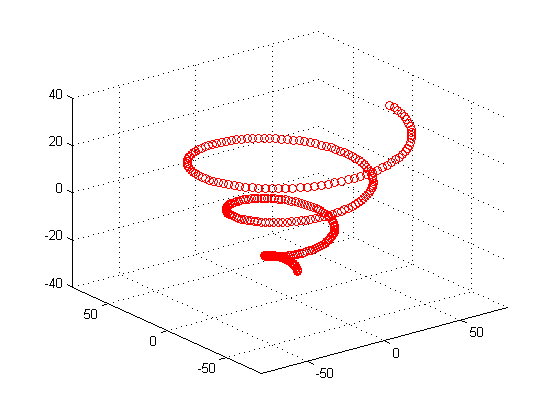
\includegraphics[width=3in,height=2.4in]{Fig/flared_helix_target}}
\caption{The simulated 3-D flared helix target distribution}
\label{fig:flared_helix_target}
\end{figure}
Before running the proposed Adaptive Annealed IS (AAIS) algorithm,
we select the initial proposal to be a T-mixture that is composed of
10 equally weighted components. The degree of freedom for each T
component is fixed to be 5. The centers of these components are
selected uniformly from a region restricted by
$x\in[-100,100],y\in[-100,100]$ and $z\in[-30,30]$. Then the
covariance matrix for every component is identical to
$\mbox{diag}[\sigma_x^2,\sigma_y^2,\sigma_z^2]$, where $\sigma_a$ is
the standard error of the argument $a$ in the components' centers
that has been just specified. The particle size $N=2000$,
$\lambda_t=0.1t$, and $t=1,\ldots,10$.

The adaptive mixture importance sampling (AMIS) approach
\cite{cappe2008ais} is involved for performance comparison. We
initialize it using the same setting as for the AAIS, and let it run
10 iterations to give the final mixture importance function.

Fig. \ref{fig:helix_scatter} shows the resulting posterior samples
(which are equally weighted via resampling) corresponding to AAIS
and AMIS, respectively. It's shown that the samples resulted from
AAIS are distributed in wider posterior area, which indicates that
the importance function given by AAIS captures more structures in
the posterior.

\begin{figure}[!htb]
\begin{tabular}{c}
\centerline{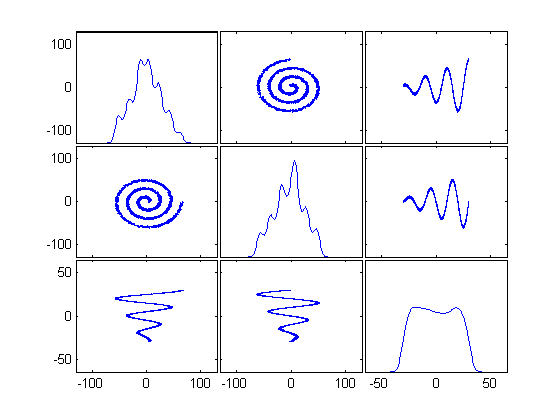
\includegraphics[width=3in,height=2.4in]{Fig/flared_helix_scatter.png}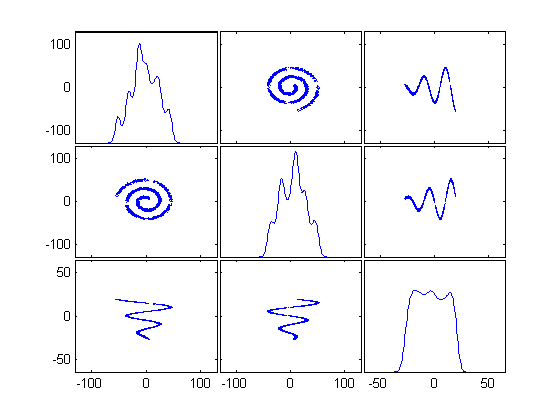
\includegraphics[width=3in,height=2.4in]{Fig/AIS_3d_felix_scatter.png}}
\end{tabular}
\caption{Three dimensional flared helix example. Left:posterior
samples produced by the proposed AAIS algorithm. Right:posterior
samples produced by the AMIS algorithm \citep{cappe2008ais}. In the
diagonal, the curves are kernel density estimates of the posterior
samples.} \label{fig:helix_scatter}
\end{figure}

A quantitative comparison between the importance functions obtained
by AAIS and AMIS is shown in Table \ref{comparison_3D}. Three
quantities are used for comparison, that are the \ESS, the KL
distance and the estimated marginal likelihood. Note that, we can
easily calculate the KL distance via a simple Monte Carlo for this
simulation case. As is shown in Table \ref{comparison_3D}, AAIS
gives correct answer to the marginal likelihood, closer KL distance
with respect to the real target, and bigger \ESS. So it further
demonstrates that the AAIS is much better than the AMIS in dealing
with this simulation case.

\begin{table}
\begin{tabular}{c||c|c|c}
 & \ESS/N & $\KL$ & Marginal Likelihood (real answer:60) \\
\hline AMIS \citep{cappe2008ais} & 0.1525 & 6.7830 & $47.2\pm3.3$\\
\hline AAIS proposed here & 0.4459 & 0.1586 & $59.7\pm2.0$\\
\hline
\end{tabular}
\caption{Three dimensional flared helix example. Quantitative
Performance comparison.}\label{comparison_3D}
\end{table}

\subsection{ Outer Product of Seven Univariate Densities}
To test the concern whether good results from a 3-D example imply
good results in higher dimensions, we used as a target function the
outer product of seven univariate distributions normalized to
integrate to 1. These seven distributions are:
\begin{enumerate}
\item $\frac{3}{5}\mathcal{G}(10+x|2,3)+\frac{2}{5}\mathcal{G}(10-x|2,5)$
\item $\frac{3}{4}sk\mathcal{N}(x|3,1,5)+\frac{1}{4}sk\mathcal{N}(x|-3,3,-6)$
\item $\mathcal{S}(x|0,9,4)$
\item $\frac{1}{2}\mathcal{B}(x+3|3,3)+\frac{1}{2}\mathcal{N}(x|0,1)$
\item $\frac{1}{2}\varepsilon(x|1)+\frac{1}{2}\varepsilon(-x|1)$
\item $sk\mathcal{N}(x|0,8,-3)$
\item $\frac{1}{8}\mathcal{N}(x|-10,0.1)+\frac{1}{4}\mathcal{N}(x|0,0.15)+\frac{5}{8}\mathcal{N}(x|7,0.2)$
\end{enumerate}
Here $\mathcal{G}(\cdot|\alpha,\beta)$ denotes the gamma
distribution, $\mathcal{N}(\cdot|\mu,\sigma)$ denotes the normal
distribution, $sk\mathcal{N}(\cdot|\mu,\sigma,\alpha)$ denotes the
skew-normal distribution, $\mathcal{S}(\cdot|\mu,s,df)$ denotes the
student-T distribution, $\mathcal{B}(\cdot|\alpha,\beta)$ denotes
the beta distribution, and $\varepsilon(\cdot|\lambda)$ denotes the
exponential distribution. Dimension 2 has two modes bracketing a
deep ravine, dimension 4 has one low, broad mode that overlaps a
second sharper mode, and dimension 7 has three distinct,
well-separated modes. Only dimension 5 is symmetric. There is a
range of tail behavior as well, from Gaussian to heavy-tailed.

In this case, we initialize the proposed AAIS algorithm with a
T-mixture that is composed of 50 equally weighted components. The
degree of freedom for each T component is still fixed to be 5. The
centers of these components for each dimension are selected
uniformly $[-10,10]$. The procedure to initialize the covariance
matrix for every mixture component is identical to that used for the
example shown in Section \ref{sec:example1}. We specify a particle
size $N=8000$, and annealing schedule $\lambda_t=0.1t$, with
$t=1,\ldots,10$.

The AMIS method \citep{cappe2008ais} is also involved for
performance comparison. The AMIS is initialized identically as for
AAIS, and will run 10 iterations to give the final result.

Fig.\ref{fig:7D_scatter} depicts the scatterplot for the resulting
posterior samples (which has been equally weighted by resampling).
It's shown that, the AMIS missed modes in the 2nd and 7th dimension,
while the proposed AAIS manages to capture all the modes in the
posterior, which should be benefited from the annealing idea being
involved.

\begin{figure}[!htb]
\begin{tabular}{c}
\centerline{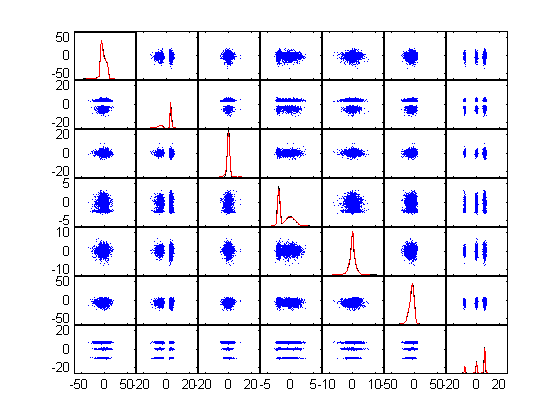
\includegraphics[width=4in,height=3.2in]{Fig/seven_outer_product_scatter.png}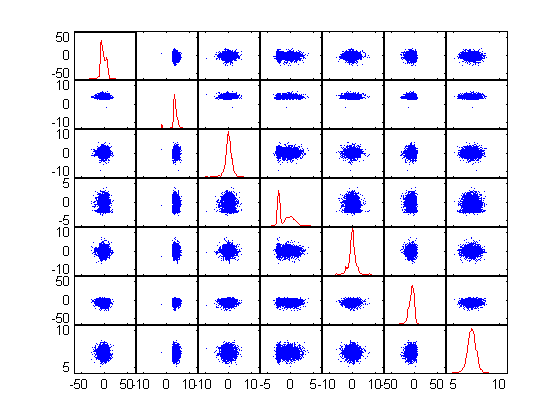
\includegraphics[width=4in,height=3.2in]{Fig/AIS_7d_outter_scatter.png}}
\end{tabular}
\caption{Seven dimensional outer product example. Left:posterior
samples produced by the proposed AAIS algorithm. Right:posterior
samples produced by the AMIS algorithm \citep{cappe2008ais}. In the
diagonal, the curves are kernel density estimates of the posterior
samples.} \label{fig:7D_scatter}
\end{figure}

Similarly as for example 1, we give a quantitative comparison for
the involved algorithms in Table \ref{comparison_7d}. We see that
again the proposed AAIS algorithm leads to much better results for
every comparison criterion.

\begin{table}
\begin{tabular}{c||c|c|c}
 & \ESS/$N$ & $\KL$ & Marginal likelihood: (true value:1) \\
\hline AMIS \citep{cappe2008ais}& 0.2454 & 10.8804 & $0.4675\pm0.0246$\\
\hline AAIS proposed here & 0.4948 & 0.4075  & $1.0011\pm0.0303$\\
\hline
\end{tabular}
\caption{Seven dimensional outer product example. Quantitative
Performance comparison}\label{comparison_7d}
\end{table}


\section{Exo-Planet Examples} \label{sec:app}
In this section, we perform the proposed AAIS method to deal with
two real RV data set.

\subsection{Star HD73526}
This data set contains 18 data components, and were claimed to
support an orbit of $190.5\pm3.0$ days \citep{tinney2003four}.
\cite{gregory2005bayesian} did a Bayesian re-analysis on this data
set using a parallel tempering MCMC algorithm, and reported three
possible orbits, with periods $127.88_{-0.09}^{+0.37}$,
$190.4_{-2.1}^{+1.8}$ and $376.2_{-4.3}^{+1.4}$ days, respectively.
\cite{gregory2005bayesian} also discussed the possibility of having
an additional planet, and reported that the Bayes factor is less
than 1 when comparing $\mathcal{M}_2$ with the $\mathcal{M}_1$.

We use the proposed AAIS algorithm to deal with $\mathcal{M}_0$,
$\mathcal{M}_1$ and $\mathcal{M}_2$, respectively. The marginal
likelihood estimation result is summarized in Table
\ref{marginal_likelihood_data1}. These estimates are reliable
indicated by their corresponding \ESS$/N$. The resulting Bayes
factors are shown in Table \ref{Bayes_factor_data1}. As indicated by
the result, this data set support the one-planet hypothesis, which
coincides the conclusions made by
\cite{tinney2003four,gregory2005bayesian}.

\begin{table}
\begin{tabular}{c|c|c}
 & Marginal Likelihood & \ESS$/N$\\
\hline $\mathcal{M}_0$ & $5.9013\times10^{-50}\pm5.1325\times10^{-52}$ & 0.9320\\
\hline $\mathcal{M}_1$ & $4.4886\times10^{-41}\pm3.2093\times10^{-42}$ & 0.5698\\
\hline $\mathcal{M}_2$ & $1.5511\times10^{-42}\pm3.2878\times10^{-43}$ & 0.3458\\
\hline
\end{tabular}
\caption{HD73526 \cite{tinney2003four} Data Case. The calculated
marginal likelihoods}\label{marginal_likelihood_data1}
\end{table}

\begin{table}
\begin{tabular}{c|c}
 \BF$\{\mathcal{M}_1:\mathcal{M}_0\}$ & \BF$\{\mathcal{M}_2:\mathcal{M}_1\}$\\
\hline $7.606\times10^8$& 0.03456\\
\hline
\end{tabular}
\caption{HD73526 \citep{tinney2003four} Data Case. The calculated
Bayes Factors}\label{Bayes_factor_data1}
\end{table}

Specifically for $\mathcal{M}_1$, we show the posterior samples
(equally weighted by resampling) in Fig. \ref{fig:scatter_1p_data1}.
 We obtain two modes in $P$, that are $P_1=190.1_{-1.5}^{+2.2}$ and
$P_2=375.5_{-2.5}^{+2.0}$, respectively.

\begin{figure}[!htb]
\centerline{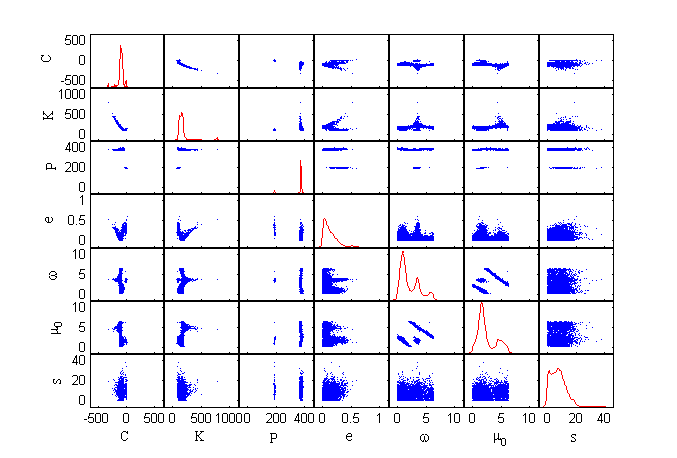
\includegraphics[width=4in,height=3.2in]{Fig/scatter_1p_data1.png}}
\caption{HD73526 \cite{tinney2003four} Data Case. Scatter plot of
the posterior samples of
$\mathcal{M}_1$}\label{fig:scatter_1p_data1}
\end{figure}

\subsection{Star HD73526}
This data set contains 30 RV data components and was claimed to have
two planets \citep{tinney20062}.

We calculate the marginal likelihoods using the proposed AAIS
algorithm, and the result is shown in Table
\ref{marginal_likelihood_data2}. Indicated by the criterion
\ESS$/N$, we deem that the result is reliable. The resulting Bayes
factors can be seen in Table \ref{Bayes_factor_data2}. So our result
supports the argument in \cite{tinney20062}$-$there are two planets
underlying this data set.

\begin{table}
\begin{tabular}{c|c|c}
 & Marginal Likelihood & \ESS$/N$\\
\hline $\mathcal{M}_0$ & $8.9566\times10^{-77}\pm1.0852\times10^{-78}$ & 0.9510\\
\hline $\mathcal{M}_1$ & $5.8519\times10^{-70}\pm1.7077\times10^{-71}$ & 0.6545\\
\hline $\mathcal{M}_2$ & $4.8122\times10^{-65}\pm1.4284\times10^{-66}$ & 0.2034 \\
\hline
\end{tabular}
\caption{HD73526 \citep{tinney20062} Data Case. The calculated
marginal likelihoods}\label{marginal_likelihood_data2}
\end{table}

\begin{table}
\begin{tabular}{c|c}
 \BF$\{\mathcal{M}_1:\mathcal{M}_0\}$ & \BF$\{\mathcal{M}_2:\mathcal{M}_1\}$\\
\hline $6.534\times10^6$& $8.233\times10^4$\\
\hline
\end{tabular}
\caption{HD73526 \citep{tinney20062} Data Case. The calculated
Bayes Factors}\label{Bayes_factor_data2}
\end{table}

The posterior samples (equally weighted by resampling) corresponding
to $\mathcal{M}_1$ is shown in Fig.\ref{fig:scatter_1p_data2}, and
the algorithm again captures two modes in $P$, that are
$P_1=193.1162_{-3.7}^{+2.1}$ and $P_2=374.8732_{-5.8}^{+6.9}$.

When dealing with $\mathcal{M}_2$, we still restrict the period of
the first planet to be smaller than that of the second planet.
Fig.\ref{fig:scatter_2p_data2} shows the posterior samples of
$\mathcal{M}_2$. Given these posterior samples, we get the periods
of the two planets, that are $P_1=187.9379_{-0.8}^{+2.1}$ and
$P_2=377.3030_{-4.5}^{+5.2}$, respectively.
\begin{figure}[!htb]
\centerline{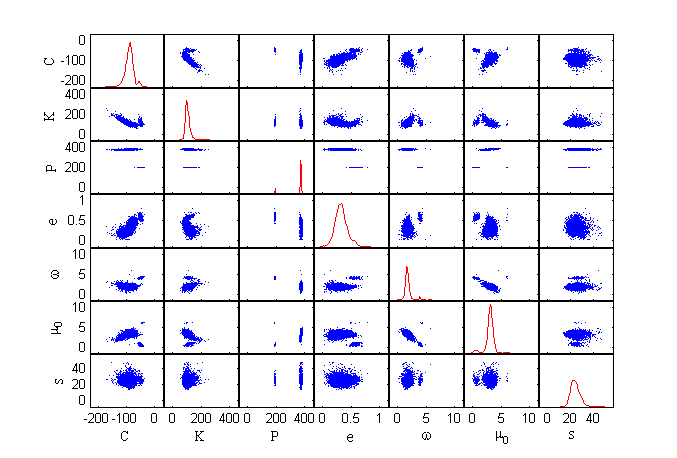
\includegraphics[width=4in,height=3.2in]{Fig/scatter_1p_data2.png}}
\caption{HD73526 \citep{tinney20062} Data Case. Scatter plot of the
posterior samples of $\mathcal{M}_1$}\label{fig:scatter_1p_data2}
\end{figure}

\begin{figure}[!htb]
\begin{tabular}{c}
\centerline{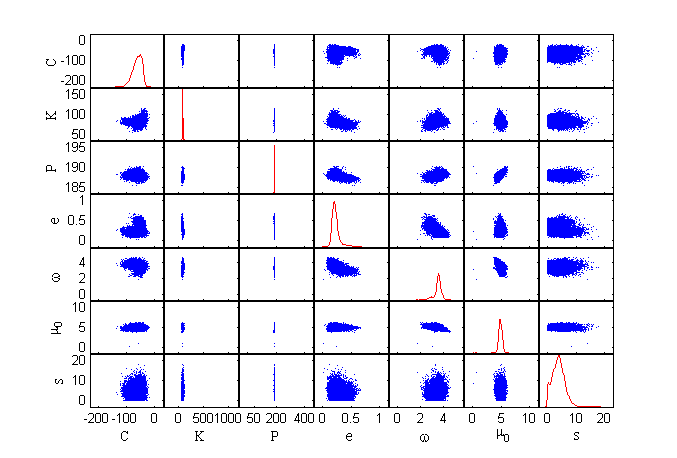
\includegraphics[width=4in,height=3.2in]{Fig/scatter1_2p_data2.png}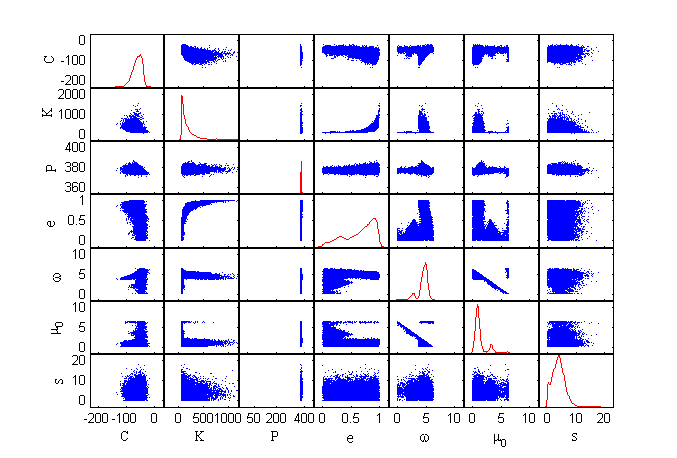
\includegraphics[width=4in,height=3.2in]{Fig/scatter2_2p_data2.png}}\\
\end{tabular}
\caption{HD73526 \cite{tinney20062} Data Case. Scatter plot of the
posterior samples of $\mathcal{M}_2$. Left: Scatter plot of the
posterior samples of the first planet parameter; Right: Scatter plot
of the posterior samples of the second planet parameter}
\label{fig:scatter_2p_data2}
\end{figure}


Given samples from the posterior, we can easily get the minimum mean
squared estimate (MMSE) of the RV at any given time, and then plot
the RV curve. In Fig.\ref{fig:rv_comparison_data2}, we plot the
estimated RV curves on basis of $\mathcal{M}_0$, $\mathcal{M}_1$ and
$\mathcal{M}_2$, respectively, meanwhile the real RV observations
are depicted there for reference. As in shown, the RV estimation
yielded by $\mathcal{M}_2$ fits the real data best.

\begin{figure}[!htb]
\centerline{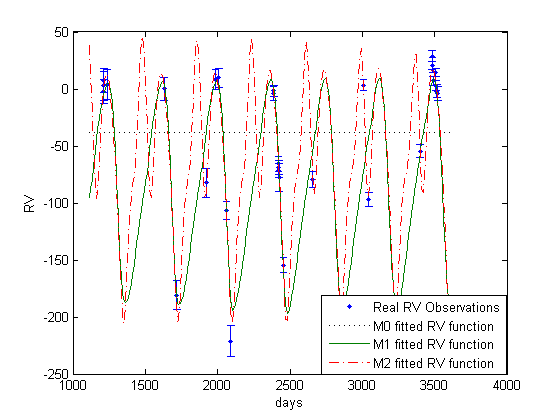
\includegraphics[width=4in,height=3.2in]{Fig/rv_comparison_data2.png}}
\caption{Measured velocities (filled circles) vs. time for HD73526
\cite{tinney20062}. Error bars only includes internal uncertainties.
The curves are MMSE estimates of the RV yielded by $\mathcal{M}_0$,
$\mathcal{M}_1$ and $\mathcal{M}_2$,
respectively}\label{fig:rv_comparison_data2}
\end{figure}

\subsection{The HD217107 Data Case}
Star HD217107 was claimed to have two planets \citep{vogt2005five}.

We analyze the observed RV data for HD217107 using our AAIS method,
the calculated marginal likelihoods are shown in Table
\ref{marginal_likelihood_HD217107}, each corresponding to a
sufficiently big value of \ESS$/N$. The resulting Bayes factors can
be seen in Table \ref{Bayes_factor_HD217107}. It's shown that
$\mathcal{M}_2$ beats both $\mathcal{M}_0$ and $\mathcal{M}_1$.

\begin{table}
\begin{tabular}{c|c|c}
 & Marginal Likelihood & \ESS$/N$\\
\hline $\mathcal{M}_0$ & $3.6492\times10^{-168}\pm7.0150\times10^{-169}$ & 0.9644\\
\hline $\mathcal{M}_1$ & $3.7389\times10^{-141}\pm0.6077\times10^{-142}$ & 0.6448\\
\hline $\mathcal{M}_2$ & $3.0897\times10^{-108}\pm1.0011\times10^{-109}$ & 0.4119 \\
\hline
\end{tabular}
\caption{HD217107 \citep{vogt2005five} Data Case. The calculated
marginal likelihoods}\label{marginal_likelihood_HD217107}
\end{table}

\begin{table}
\begin{tabular}{c|c}
 \BF$\{\mathcal{M}_1:\mathcal{M}_0\}$ & \BF$\{\mathcal{M}_2:\mathcal{M}_1\}$\\
\hline $1.025\times10^{27}$& $8.264\times10^{32}$\\
\hline
\end{tabular}
\caption{HD217107 \citep{vogt2005five} Data Case. The calculated
Bayes Factors}\label{Bayes_factor_HD217107}
\end{table}

\subsection{The HD37124 Data Case}
Star HD37124 was claimed to have three planets \citep{vogt2005five}.

We analyze the associated RV data set using our AAIS method, the
marginal likelihoods calculated by our AAIS algorithm are shown in
Table \ref{marginal_likelihood_37124}. Indicated by the criterion
\ESS$/N$, the results are reliable. The resulting Bayes factors can
be seen in Table \ref{Bayes_factor_37124}, which support the
conclusion of \cite{tinney20062}, i.e. this data set supports the
three-planet hypothesis.

\begin{table}
\begin{tabular}{c|c|c}
 & Marginal Likelihood & \ESS$/N$\\
\hline $\mathcal{M}_0$ & $2.0889\times10^{-110}\pm2.1857\times10^{-112}$ & 0.9427\\
\hline $\mathcal{M}_1$ & $1.0717\times10^{-106}\pm1.3077\times10^{-107}$ & 0.1737\\
\hline $\mathcal{M}_2$ & $1.9830\times10^{-97}\pm1.1451\times10^{-98}$ & 0.1798 \\
\hline $\mathcal{M}_3$ & $2.9228\times10^{-84}\pm1.2563\times10^{-85}$ & 0.1305 \\
\hline
\end{tabular}
\caption{HD37124 \citep{vogt2005five} Data Case. The calculated
marginal likelihoods}\label{marginal_likelihood_37124}
\end{table}

\begin{table}
\begin{tabular}{c|c|c}
\BF$\{\mathcal{M}_1:\mathcal{M}_0\}$ &\BF$\{\mathcal{M}_2:\mathcal{M}_1\}$ & \BF$\{\mathcal{M}_3:\mathcal{M}_2\}$\\
\hline $5.13\times10^3$ & $1.850\times10^9$ & $1.474\times10^{13}$\\
\hline
\end{tabular}
\caption{HD37124 \citep{vogt2005five} Data Case. The calculated
Bayes Factors}\label{Bayes_factor_37124}
\end{table}

In Fig.\ref{fig:hd37124_fit}, we plot the estimated RV curves on
basis of $\mathcal{M}_1$, $\mathcal{M}_2$ and $\mathcal{M}_3$,
respectively, where the real RV observations is also depicted for
reference. As is shown, the RV estimation yielded by $\mathcal{M}_3$
fits the real data best.



\begin{figure}[!htb]
\begin{tabular}{c}
\centerline{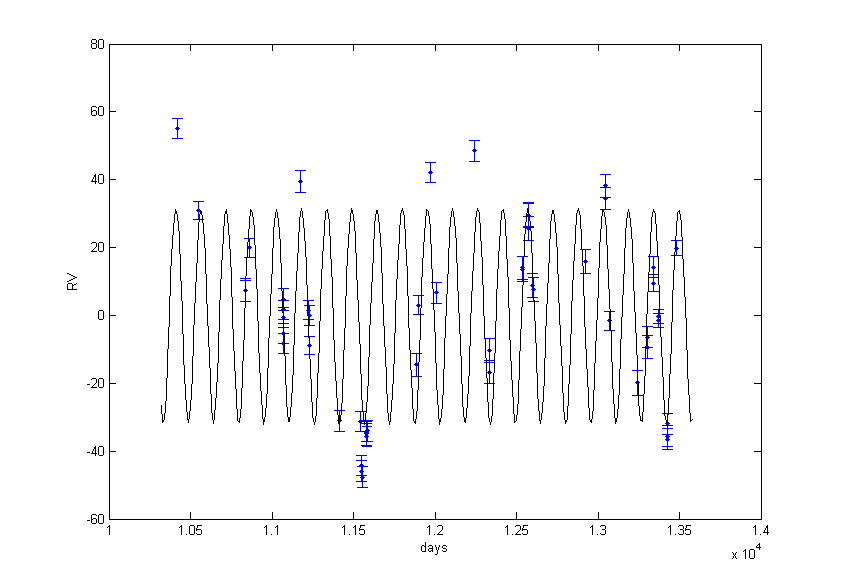
\includegraphics[width=4in,height=3.2in]{Fig/hd37124_1p_fit.png}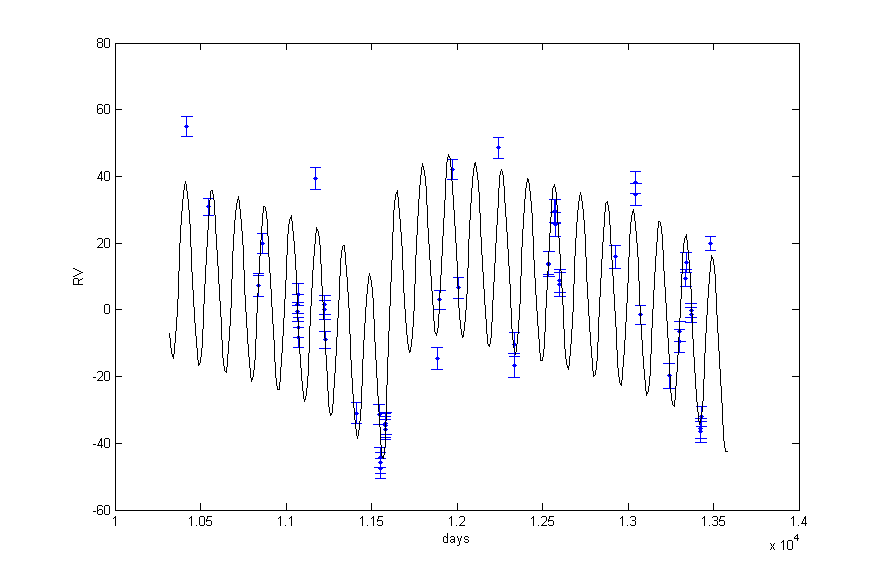
\includegraphics[width=4in,height=3.2in]{Fig/hd37124_2p_fit.png}}\\
\centerline{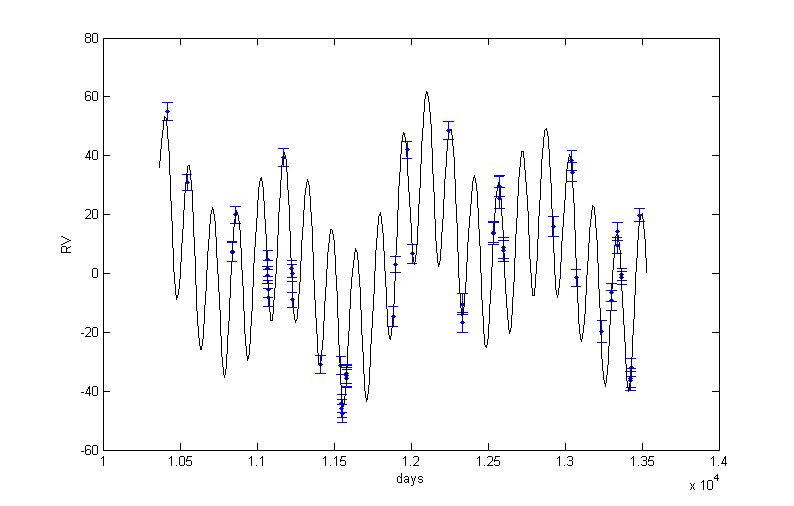
\includegraphics[width=4in,height=3.2in]{Fig/hd37124_3p_fit.png}}
\end{tabular}
\caption{Measured velocities (filled circles) vs. time for HD37124
\cite{tinney20062}. Error bars only includes internal uncertainties.
The MMSE estimates of the RV curves yielded by using
$\mathcal{M}_1$, $\mathcal{M}_2$ and $\mathcal{M}_3$ are shown in
the top left, top right and the bottom panels, respectively.}
\label{fig:hd37124_fit}
\end{figure}

\subsection{The 47 Ursae Majoris (47 UMa) Data Case}
This 47 UMa data recently was analyzed in
\cite{gregory2010bayesian}.

We analyze the associated RV data set using our AAIS method, the
marginal likelihoods calculated by our AAIS algorithm are shown in
Table \ref{marginal_likelihood_uma47}. We obtain reliable estimates
for $\mathcal{M}_0$, $\mathcal{M}_1$ and $\mathcal{M}_2$, while the
estimate for $\mathcal{M}_3$ is unreliable, the \ESS$/N$ is 0.0089,
which is not big enough. Indicated by the criterion \ESS$/N$, the
results are reliable. So we argue that this data set supports
$\mathcal{M}_2$ more than $\mathcal{M}_0$ and $\mathcal{M}_1$, but
we are not sure about the relative strength between $\mathcal{M}_2$
and $\mathcal{M}_3$. \cite{gregory2010bayesian} concluded that this
data set has three planets, however, gave an much ambiguous estimate
for the third planet's period.

\begin{table}
\begin{tabular}{c|c|c}
 & Marginal Likelihood & \ESS$/N$\\
\hline $\mathcal{M}_0$ & $2.0198\times10^{-1004}\pm9.2572\times10^{-1006}$ & 0.1002\\
\hline $\mathcal{M}_1$ & $3.4400\times10^{-896}\pm3.10\times10^{-897}$ & 0.5643\\
\hline $\mathcal{M}_2$ & $1.3500\times10^{-816}\pm1.77\times10^{-817}$ & 0.3324 \\
\hline $\mathcal{M}_3$ & $2.8970\times10^{-825}\pm9.1623\times10^{-825}$ & 0.0089 \\
\hline
\end{tabular}
\caption{uma47 \citep{gregory2010bayesian} Data Case. The
calculated marginal likelihoods}\label{marginal_likelihood_uma47}
\end{table}

\begin{table}
\begin{tabular}{c|c|c}
 \BF$\{\mathcal{M}_1:\mathcal{M}_0\}$ & \BF$\{\mathcal{M}_2:\mathcal{M}_1\}$ & \BF$\{\mathcal{M}_3:\mathcal{M}_2\}$\\
\hline $1.703\times10^{108}$ & $3.924\times10^{79}$ & $ ?$\\
\hline
\end{tabular}
\caption{uma47 \citep{gregory2010bayesian} Data Case. The
calculated Bayes Factors}\label{Bayes_factor_uma47}
\end{table}

In Fig.\ref{fig:uma47_fit}, we plot the estimated RV curves on basis
of $\mathcal{M}_1$, $\mathcal{M}_2$ respectively, and again the real
RV observations are depicted there for reference. As is shown, the
RV estimation yielded by $\mathcal{M}_2$ fits better.

\begin{figure}[!htb]
\begin{tabular}{c}
\centerline{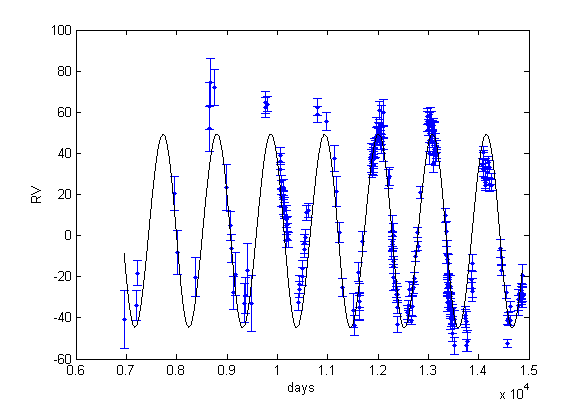
\includegraphics[width=4in,height=3.2in]{Fig/uma47_1p_fit.png}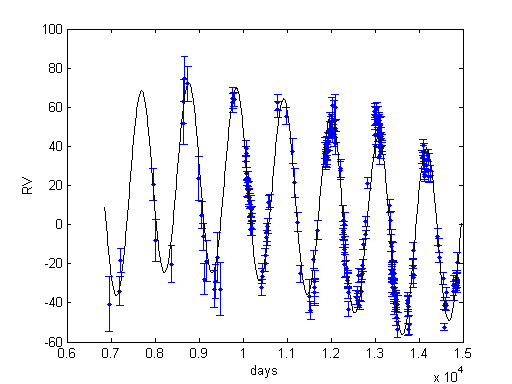
\includegraphics[width=4in,height=3.2in]{Fig/uma47_2p_fit.png}}
\end{tabular}
\caption{Measured velocities (filled circles) vs. time for the 47
Ursae Majoris (47 UMa) \citep{gregory2010bayesian}. Error bars only
includes internal uncertainties. The MMSE estimates of the RV curves
yielded by using $\mathcal{M}_1$ and $\mathcal{M}_2$ are shown in
the left and the right panels, respectively.} \label{fig:uma47_fit}
\end{figure}



\section{Discussions and Conclusions} \label{sec:disc}
In this paper, we propose an adaptive mixture modeling approach to
construct importance function for IS. The resulting mixture model is
demonstrated to be capable of capturing separated peaky structures
in the posterior, even when it is high-dimensional (an at most
17-dimensional posterior is considered in this paper).
Straightforwardly, this approach facilitates simulating draws from
multi-modal joint posterior distribution by IS, and provides an
effective and easy-to-implement way for estimating marginal
likelihood that is required for Bayesian model comparison.


\bibliographystyle{imsart-nameyear}
\bibliography{sais_bib}
\end{document}
